\chapter{Fast-ion Diagnostics}\label{chap:diagnostics}
There are basically two ways diagnostics can probe the fast-ion distribution. The first is to directly collect samples from the distribution. Direct sampling of the distribution is difficult because any probe inserted into the plasma would not survive due to the highly corrosive environment of a fusion plasma. Because of this, samples can only be drawn from the very edge of the plasma where the environment is more friendly to diagnostics. This effectively limits the types of fast ions detected. Case in point, one of the few direct fast-ion diagnostics, the fast-ion loss detector (FILD), only measures---as the name suggests---fast-ions that are lost to the wall---a useful diagnostic but limited in the information gained about the fast-ion distribution as a whole.

A different approach to fast-ion diagnostics is to measure the byproducts of their interactions with the plasma. This approach allows for more information about the fast-ion distribution to be gained. However, the increased information comes at a cost. Since the diagnostics do not directly measure the fast ions, we must model what the detector would measure for any given fast-ion---we call this the diagnostic's forward model. Even though we have more information about the fast-ion distribution, it is garbled by the diagnostic's forward model. This makes the analysis of our data difficult. In experiment, we only ever see the noisy output of the forward model. In order to validate a theoretical distribution function, we have to run the distribution through the diagnostic's forward model to get an apples to apples comparison with data. This is not an ideal scenario. Fortunately, as we will see in Chapters \ref{chap:velocity-space_tomography}-\ref{chap:orbit_tomography}, it is possible to reverse this process to obtain the fast-ion distribution from measurement alone. In order to do this, we need the forward model of our diagnostics.

In the following sections, we will discuss three different fast-ion diagnostics and their forward models: Neutral Particle Analyzers (NPA), Fast-ion D-$\alpha$ spectroscopy (FIDA), and neutron scintillators.

\section{Neutral Particle Analyzers}
\begin{figure}[ht]
    \centering
    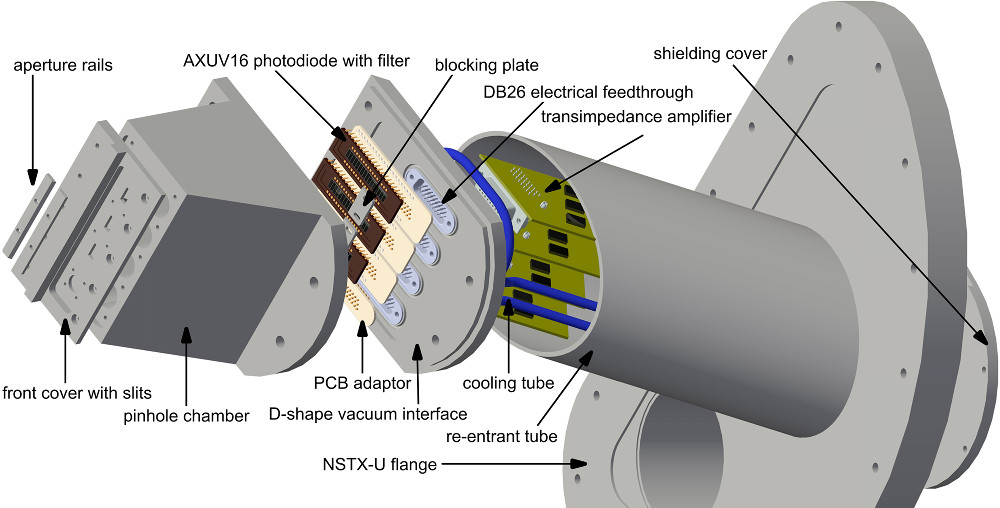
\includegraphics[width=12cm]{figures/nstx_npa.jpeg}
    \caption{Expanded view of NSTX-U's solid state neutral particle analyzer array.\cite{liu2014design}}
    \label{fig:npa}
\end{figure}
Neutral particle analyzers detect fast ions that have undergone a charge exchange (CX) reaction with a neutral population within the plasma, becoming a fast neutral. Since the fast neutral is not confined by the magnetic field, information about the fast ions in the center of the plasma can be attained. Neutral particle analyzers were one of the first fast-ion diagnostics\cite{artsimovich1969experiments}. However, in recent years there has been a bit of a renaissance in their design. Compact solid state analyzers\cite{zhu2012compact} allowed for more sightlines in a smaller space. This type of design has recently been installed on NSTX-U (Fig. \ref{fig:npa}). Most recently, an Imaging NPA that combines the best aspects of traditional analyzers and fast-ion loss detectors has been deployed at DIII-D, showing excellent initial results\cite{du2018inpa}.

\subsection{Forward Model of the Neutral Particle Analyzer}
As mentioned, neutral particle analyzers detect fast neutrals that are born of charge exchange reactions with the neutral populations within the tokamak, in which there are several.
Neutral beam injection creates three distinct neutral populations due to the acceleration of molecular hydrogen.
During the neutralization phase of neutral beam injection, the molecular forms of hydrogen are eliminated and the gained energy is split evenly among the atoms.
The energy of each population is given by $E_i = E_1/i$, where $i$ is the number of hydrogen atoms in each molecule.
The velocity distribution of each species is tightly focused and can be approximated by a Dirac delta function.
A fourth population of neutrals forms when injected neutrals charge exchange with thermal ions, creating a thermal ``halo'' with a shifted Maxwellian velocity distribution. A fifth type of neutral occur when thermal ions reach the cold edge of the plasma and neutralize. This creates a cold edge neutral population that has a shifted Maxwellian velocity distribution. These cold edge neutrals are always present and are independent of the neutral beam. Since certain signals are only present when the neutral beam is on, we tend to separate the signals that come from CX with the beam (active signals) and signals that originate from CX with the cold edge neutrals (passive signals), although the following derivation of the forward model makes no such distinction.

Consider a beam of fast ions traveling through a cloud of neutral particles. The fast ions can undergo the following charge exchange reaction to create a fast neutral,
\begin{equation}
    H_f^+ + H(m) \rightarrow H_f(n) + H^+\,,
\end{equation}
where $H_f^+$ is the fast ion, $H(m)$ is the donor neutral in energy state $m$, $H_f(n)$ is the fast neutral in energy state $n$, and $H^+$ is the newly created ion.
The rate in which the fast ion, when interacting with the $k$ different neutral populations, produces a fast neutral in a given energy level is given by
\begin{equation}\label{eq:cx_rates}
    \mathbf{f}(t=0) = \sum_k \left [ \int \mathbf{X}(\mathbf{v}_f - \mathbf{v}) \cdot \mathbf{d}_k\, ||\mathbf{v}_f - \mathbf{v}||\, f_k(\mathbf{v})\, d\mathbf{v} \right ]\,,
\end{equation}
where $\mathbf{X}$ $[cm^2]$ is a $n \times m$ matrix of the charge exchange cross sections, $\mathbf{d}_k$ $[cm^{-3}]$ is the densities vector of the $m$ energy levels of the donor neutral, and $f_k$ is the velocity distribution of the $k^{th}$ neutral population. This is called the neutral population flux.
The neutral population flux, $\mathbf{f}$, evolves in time as it travels through the background plasma due to collisions with the different plasma species, the most significant collisions being:
\begin{itemize}
    \item excitation and/or ionization with electrons,
    \item excitation and/or ionization with ions,
    \item charge exchange with ions.
\end{itemize}

The effects of the different collisional processes on the population flux can be modeled by the following matrix differential equation 
\begin{equation}\label{eq:colrad}
    \frac{d \mathbf{f}}{dt} = \mathbf{C} \cdot \mathbf{f}\,,
\end{equation}
where $\mathbf{C}$ is a matrix of the rate coefficients for the collisional and atomic transitions.
The full derivation of Equation \ref{eq:colrad} is given in Appendix \ref{app:colrad}.

The solution of Equation \ref{eq:colrad} takes the form of a matrix exponential,
\begin{equation} \label{eq:neutral_flux}
    \mathbf{f}(t) = e^{\mathbf{C} t} \cdot \mathbf{f}(t=0) = \mathbf{S} \cdot e^{\mathbf{\Lambda} t} \cdot \mathbf{S}^{-1} \cdot \mathbf{f}(0)\,,
\end{equation}
where $\mathbf{f}(t)$ is a vector of the neutral population flux [1/s] at time $t$, $\mathbf{S}$ is the matrix of the eigenvectors of $\mathbf{C}$ and $\mathbf{\Lambda}$ is a diagonal matrix containing the eigenvalues of $\mathbf{C}$.
Equation \ref{eq:colrad} depends on the local plasma parameters and is solved iteratively along the trajectory of the neutral. Figure \ref{fig:f_evolution} shows the evolution of the neutral population fluxes for two initial states: $f_1 = 1.0$ and $f_3=1$ with all other level populations set to zero. Despite the different initial conditions, the population fluxes trend toward an equilibrium. The time it takes to equilibrate depends on the initial states and the plasma parameters: the $f_1=1$ case equilibrates quickly and the $f_3=1$ case slowly. In experiment, the $f_1$ level is the most populated; therefore, we expect the evolution of the population flux to be closer the $f_1=1$ case.
\begin{figure}[ht]
    \centering
    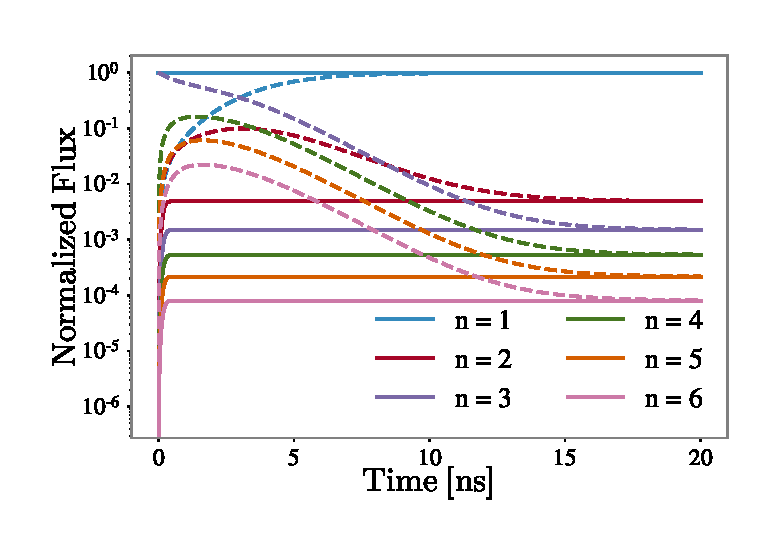
\includegraphics[width=10cm]{figures/f_evolution.eps}
    \caption{Evolution of the neutral population fluxes for two different initial conditions: $f_1=1$ (solid lines) and $f_3=1$ (dashed lines). Plasma parameters are held constant over time: $n_e = 6\times10^{13}\;cm^{-3}$, $T_e=T_i = 2\;keV$, and $Z_{eff} = 1.5$. At each time, the fluxes are normalized such that $\sum_i f_i = 1$.}
    \label{fig:f_evolution}
\end{figure}

Should the trajectory of the neutral particle enter the detector, the expected NPA signal for a fast ion with coordinates, $\mathbf{x}$, is given by
\begin{equation}\label{eq:npa_weight}
    S_{NPA}(\mathbf{x}) = \epsilon(E) \sum_n \mathbf{f}(t_{det})\,,
\end{equation}
where $t_{det}$ is the travel time to the detector and $\epsilon(E)$ is an energy dependent detector efficiency.

\section{Fast-ion D-$\alpha$ Spectroscopy}
\begin{figure}[ht]
    \centering
    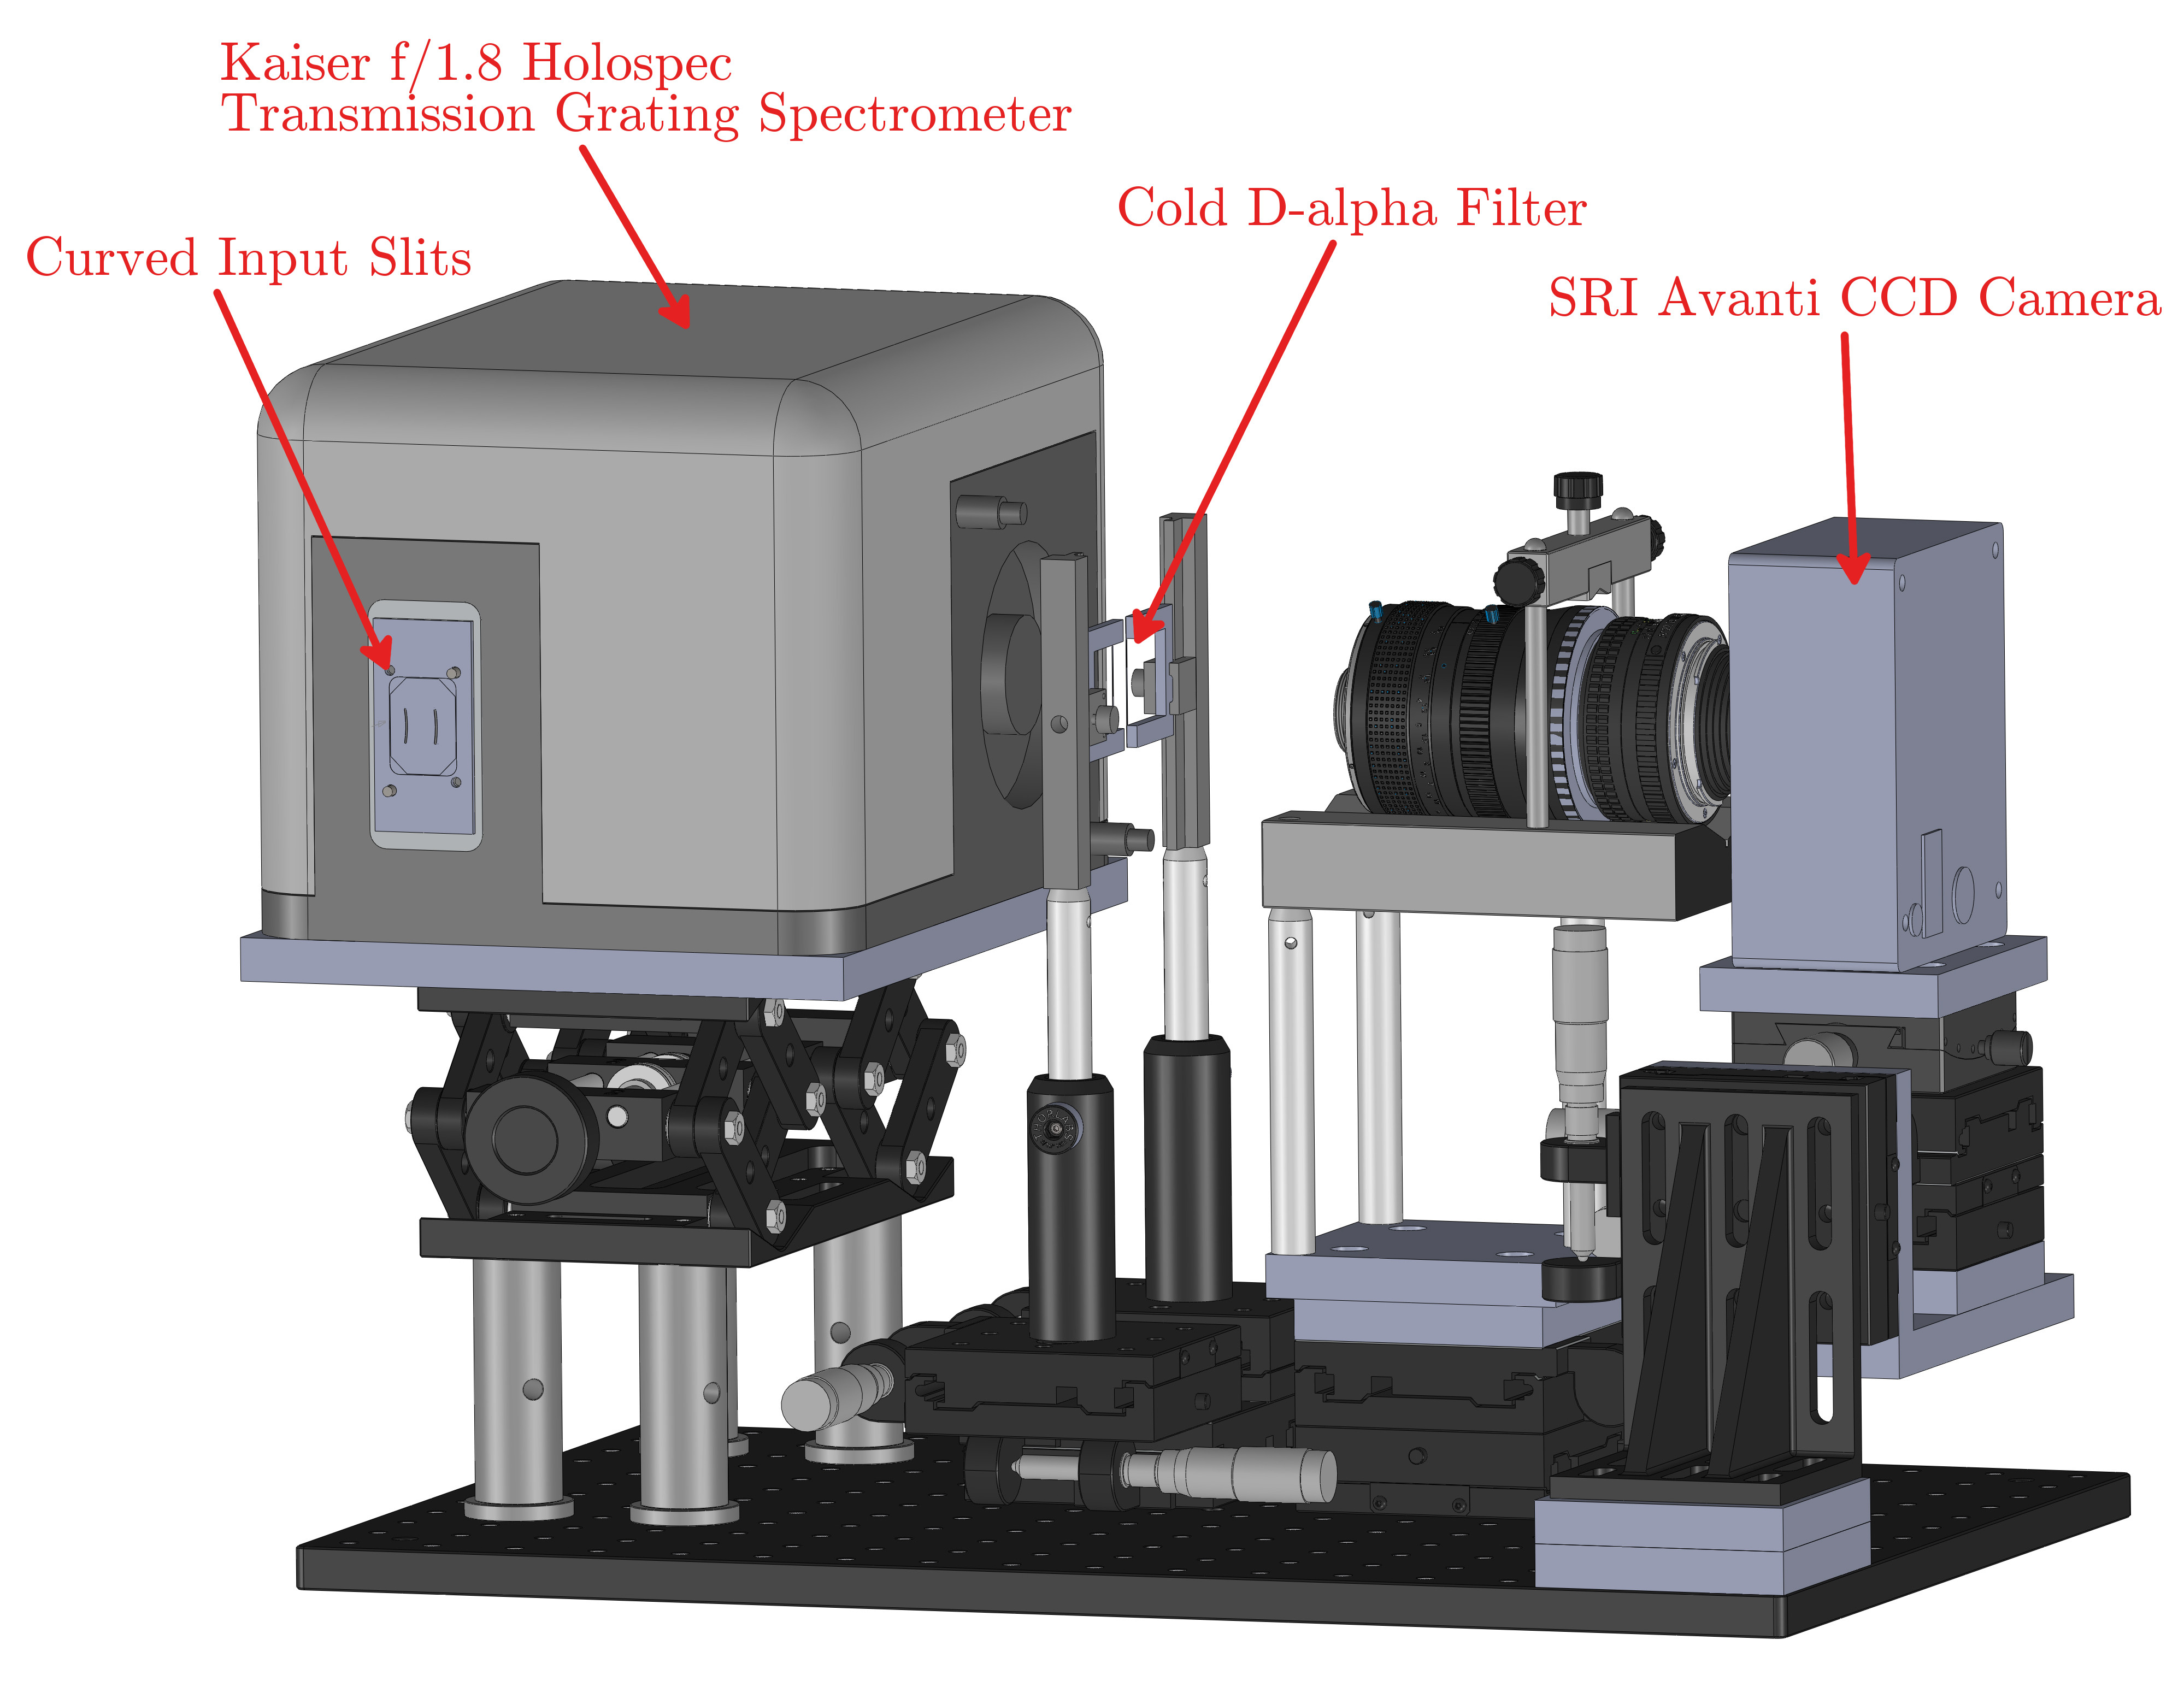
\includegraphics[width=12cm]{figures/d3d_fida.jpg}
    \caption{DIII-D's FIDA spectrometer\cite{muscatello2010}. Photons from the vessel travel through 33 optical fibers, 8 of which enter the spectrometer via input slits. The number of lines-of-sight are limited by the amount of available space on the CCD chip. To prevent saturation of the camera, the cold D-$\alpha$ emission is attenuated by a filter. Figure courtesy of Cami Collins}
    \label{fig:fida}
\end{figure}
Like the NPA diagnostic, charge exchange with a neutral population forms the basis for the Fast-ion D-$\alpha$ (FIDA) diagnostic\cite{heidbrink2004fida}. Where the NPA diagnostic measured neutrals, the FIDA diagnostic measures photons. When the fast neutral is created, it can be born in the excited $n=3$ state. As the fast neutral travels through the plasma, it will relax into the lower $n=2$ state and emit a photon. The Doppler shift of the photon contains information about the fast ion before it was neutralized. Unlike the NPA diagnostic, the bulk of the FIDA diagnostic (the spectrometer, filters, and camera) is stored away from the machine. Figure \ref{fig:fida} shows DIII-D's FIDA diagnostic which is kept in a separate room from the machine; fiber optic lines carry the emitted light from the vessel to the spectrometer. In addition to detecting FIDA light, the diagnostic also detects thermal emission from the cold edge neutrals, neutral beam emission, and Oxygen V/Carbon II impurity emission. This complicates the design and analysis of the diagnostics. For instance, the line of sight geometry must be designed to cleanly separate the FIDA signal from the contaminating sources. Despite this complication, the FIDA diagnostic has become a standard fast-ion diagnostic with implementations at most major tokamaks\cite{heidbrink2010fast}.

\subsection{Forward Model of the Fast-ion D-$\alpha$ diagnostic}
After a fast-ion charges exchanges with a neutral---the physics of which is identical to the NPA diagnostic---the resultant fast neutral can be born in an excited state. As it travels, the fast neutral will emit photons, the amount of which depends on the neutral population.
The neutral population after a time $t$, $\mathbf{n}(t)$, is found by integrating Equation \ref{eq:neutral_flux},
\begin{equation}\label{eq:neutral_population}
    \mathbf{n}(t) = \mathbf{S} \cdot ( \mathbf{\Lambda}^{-1} \cdot e^{\mathbf{\Lambda} t} - \mathbf{\Lambda}^{-1} ) \cdot \mathbf{S}^{-1} \cdot \mathbf{f}(0).
\end{equation}
If $t$ represents the time spent inside a measurement volume, $V$, the Balmer-$\alpha$ photon flux is given by
\begin{equation}\label{eq:photon_flux}
    \Phi_\gamma = n_{3}(t)\,A_{3 \rightarrow 2}\,
\end{equation}
where $A_{3\rightarrow2}$ is the spontaneous emission rate for the D-$\alpha$ transition.
The photon radiance can then be calculated by integrating the photon flux density per steradian over the line of sight,
\begin{equation}\label{eq:photon_radiance}
    L_\gamma = \frac{1}{4\pi V} \int_{LOS} \Phi_\gamma\, dl .
\end{equation}

In the presence of a magnetic field, the motion of an ion will induce an electric field, breaking the spherical symmetry of the atom.
This allows for the existence of multiple stable states that have the same principle quantum number $n$.
This effect is called Motional Stark splitting.
In this case, it is simpler to use parabolic coordinates, $|k_1,k_2,m\rangle$, instead of the usual $|n,l,m\rangle$ spherical coordinates to solve for the perturbed energy levels of the Hydrogen atom. The parabolic coordinates are related to the spherical coordinates through the relation: $n = k_1 + k_2 + |m| + 1$.
For hydrogenic atoms, the energy difference between the different stark states is proportional to the electric field strength and is given by
\begin{equation}\label{eq:stark_splitting}
    \Delta \mathcal{E}(n,k_1,k_2) = \frac{3\,n\,E\,a_0}{2}\,(k_1 - k_2) \quad [\mathrm{eV}]\,,
\end{equation}
where $a_0$ is the Bohr radius and $E$ is the magnitude of the induced electric field\cite{bethe&salpeter}. Figure \ref{fig:stark_splitting} shows the splitting and possible transitions for the $n=3\rightarrow2$ transition.
\begin{figure}[ht]
    \centering
    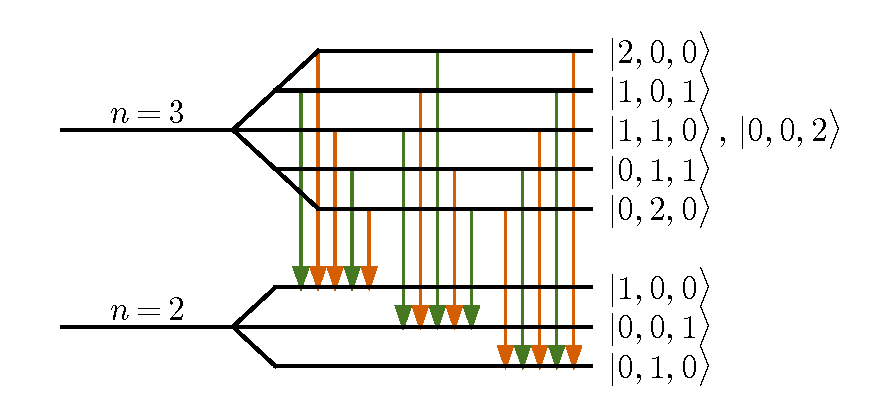
\includegraphics[width=10cm]{stark_splitting.eps}
    \caption{Stark splitting of the $n=3$ and $n=2$ energy levels of hydrogen. Higher levels indicate higher energy. States are labeled in parabolic coordinates $|k_1,k_2,|m|\rangle$. Possible transitions between states are indicated by arrows: green for $\sigma$ lines and orange for $\pi$ lines.}
    \label{fig:stark_splitting}
\end{figure}

As can be seen from Figure \ref{fig:stark_splitting}, there are $2n-1$ stark states for each principle quantum number, leading to 15 distinct transitions from the $n=3 \rightarrow 2$ state. The wavelength shift from the D-$\alpha$ line for the transition $|k_1,k_2,m\rangle \rightarrow |k_1',k_2',m'\rangle$ can be derived via the Taylor expansion of the Rydberg equation and is given by
\begin{equation}\label{eq:stark_lambda}
    \Delta \lambda(|k_1,k_2,m\rangle \rightarrow |k_1',k_2',m'\rangle) = \frac{3 \lambda_{0}^2\,a_0 (3(k_1-k_2) - 2(k_1' - k_2'))}{2hc} E \quad \rm{[nm]}\,,
\end{equation}
where $\lambda_0$ is the unshifted wavelength (656.1 nm).
Taking into account the Doppler shift due to the line of sight geometry, the wavelength for each Stark line is,
\begin{equation}\label{eq:wavelengths}
    \lambda(T) = \lambda_0 (1 + \Delta \lambda(T)/\lambda_0 + (\boldsymbol{\hat{\omega}} \cdot \mathbf{v}_f)/c)\,,
\end{equation}
where $T =|k_1,k_2,m\rangle \rightarrow |k_1',k_2',m'\rangle$ and $\boldsymbol{\hat{\omega}}$ is a unit vector pointing toward the collection optics. The net effect of the Doppler and Stark shifts are shown in Figure \ref{fig:stark_doppler}.
\begin{figure}[ht]
    \centering
    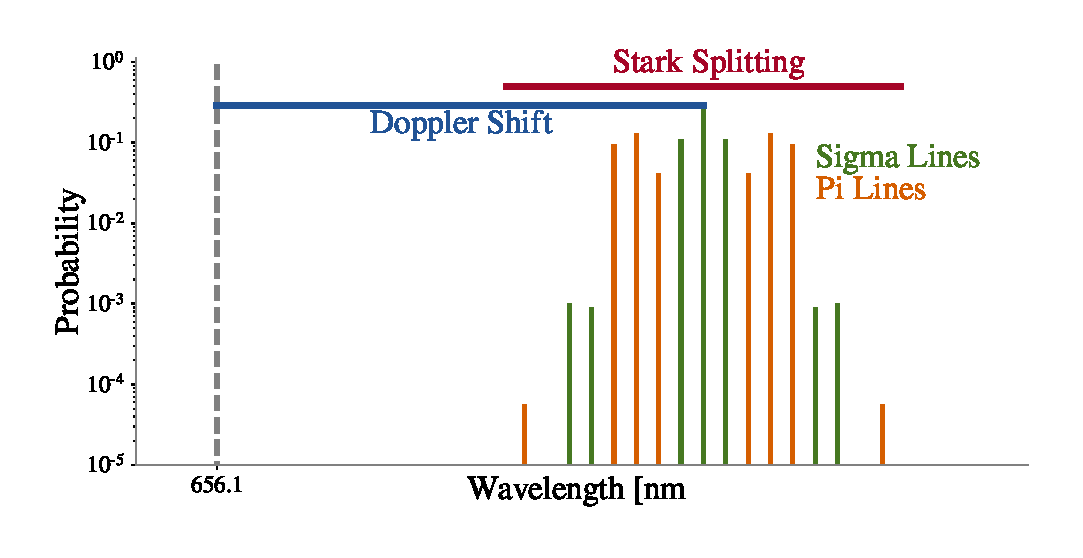
\includegraphics[width=10cm]{stark_doppler.eps}
    \caption{Doppler shift and Stark splitting on the D-$\alpha$ line. Stark line intensities are given in table \ref{tab:stark}.}
    \label{fig:stark_doppler}
\end{figure}

The photon radiance (Eq. \ref{eq:photon_radiance}) is distributed among the Stark lines.
The relative radiance of each Stark line is given by
\begin{equation}\label{eq:stark_intens}
I(T) = \epsilon(T) A(T)\,(1 \pm (\boldsymbol{\hat{\omega}} \cdot \mathbf{E})^2)\,,
\end{equation}
where $A(T)$ is the probability of transition $T$ and $\epsilon(T)$ is the diagnostic efficiency of the transition. The relative probabilities for each transition is given in Table \ref{tab:stark}. The expression in the parenthesis of Equation \ref{eq:stark_intens} is the angular distribution of the emission, which depends on the polarization of the transition: the plus sign for transitions that are linearly polarized \textit{perpendicular} to the electric field ($\sigma$ lines) and the minus sign for transitions that are linearly polarized \textit{parallel} to the electric field ($\pi$ lines).
Combining equations \ref{eq:photon_radiance}, \ref{eq:wavelengths}, and \ref{eq:stark_intens} gives the expected signal produced by a single fast ion with coordinates $\mathbf{x}$,
\begin{equation}\label{eq:fida_weight}
    S_{FIDA}(\lambda;\mathbf{x}) = \sum_T L_{\gamma}\, \frac{I(T)}{\sum_T I(T)} \delta(\lambda - \lambda(T)) \,.
\end{equation}
\begin{table}[ht]
\centering
\caption{Stark transitions and relative probabilities\cite{bethe&salpeter}. Transitions are given in parabolic coordinates. Degenerate initial states double the relative probability.}
\label{tab:stark}
\bgroup
\def\arraystretch{1.52}
\begin{tabular}{clr}
\textbf{Symbol} & \multicolumn{1}{c}{\textbf{Transition}} & \multicolumn{1}{c}{\textbf{$\mathbf{A_{rel}}$}} \\ \hline \hline
$\pi_{-7}$ & $|2,0,0\rangle \quad\! \rightarrow |0,1,0\rangle$ & $1$ \\
$\sigma_{-6}$ & $|2,0,0\rangle \quad\! \rightarrow |0,0,\pm1\rangle$ & $18$ \\
$\sigma_{-5}$ & $|1,0,\pm1\rangle \rightarrow |0,1,0\rangle$ & $2\times8$ \\
$\pi_{-4}$ & $|2,0,0\rangle\quad\! \rightarrow |1,0,0\rangle$ & $1681$ \\
$\pi_{-3}$ & $|1,0,\pm1\rangle \rightarrow |0,0,\pm1\rangle$ & $2\times1152$ \\
$\pi_{-2}$ & $|1,1,0\rangle \quad\!\rightarrow |0,1,0\rangle$ & $729$ \\
$\sigma_{-1}$ & $|1,0,\pm1\rangle \rightarrow |1,0,0\rangle$ & $2\times968$ \\
$\sigma_0$ & \begin{tabular}[l]{@{}l@{}}$|1,1,0\rangle \quad\!\rightarrow |0,0,\pm1\rangle$\\ $|0,0,\pm2\rangle \rightarrow |0,0,\pm1\rangle$\end{tabular} & \begin{tabular}[r]{@{}r@{}}$882$\\ $2\times2304$\end{tabular} \\
$\sigma_1$ & $|0,1,\pm1\rangle \rightarrow |0,1,0\rangle$ & $2\times968$ \\
$\pi_2$ & $|1,1,0\rangle\quad\! \rightarrow |1,0,0\rangle$ & $729$ \\
$\pi_3$ & $|0,1,\pm1\rangle \rightarrow |0,0,\pm1\rangle$ & $2\times1152$ \\
$\pi_4$ & $|0,2,0\rangle\quad\! \rightarrow |0,1,0\rangle$ & $1681$ \\
$\sigma_5$ & $|0,1,\pm1\rangle \rightarrow |1,0,0\rangle$ & $2\times8$ \\
$\sigma_6$ & $|0,2,0\rangle\quad\! \rightarrow |0,0,\pm1\rangle$ & $18$ \\
$\pi_7$ & $|0,2,0\rangle\quad\! \rightarrow |1,0,0\rangle$ & $1$
\end{tabular}
\egroup
\end{table}

\section{Neutron Scintillator}
As the name suggests, neutron scintillators detect the neutrons produced by fusion reactions. The name originates from the scintillating material at the heart of the detector. As a neutron passes through a scintillating material, it will produce a flash of light that a photomultiplier will turn into a electrical current---the greater the current, the greater the neutron flux. Unlike other diagnostics that look at a particular point in the plasma, uncollimated neutron scintillators, due to the highly non-interacting neutrons, detect neutrons from the whole device. Because of this, the neutron signal is a useful measure of total fast-ion confinement.

\subsection{Forward Model of a Neutron Scintillator}
A neutron can be produced via the following fusion reactions:
\begin{equation}\label{eq:D_D}
\begin{split}
    &D + D \rightarrow He^3 + n\\
    &D + T \rightarrow \alpha + n
\end{split}
\end{equation}
The total cross section for a reaction is given by
\begin{equation}
        \sigma_T(E) = \frac{S(E)}{E\exp(B_G/\sqrt{E})}\,,
\end{equation}
where $E$ is the energy in the center-of-mass frame in keV, and $B_G$ is the reactions Gamov constant. $S(E)$ is a Pad\'{e} expansion of the astrophysical S-function, which takes the approximate form\cite{bosch1992,mfeformulary}
\begin{equation}\label{eq:bosch_hale}
    S(E) = \frac{A_1 + E(A_2 + E(A_3 + E(A_4 + E A_5)))}{1 + E(B_1 + E(B_2 + E(B_3 + E B_4)))}\,,
\end{equation}
where $A$ and $B$ are coefficients. The coefficients for Equation \ref{eq:bosch_hale}, as well as the Gamov constants, are given in Table \ref{tab:bosch_hale} and the cross sections are shown in Figure \ref{fig:scattering}.
There are three sub-categories of fusion reactions that occur in a tokamak: thermonuclear fusion, where the thermal ions are fusing; beam-beam fusion, where the fast ions are fusing with themselves; and beam-plasma fusion, where the fast-ions are fusing with the thermal ions. Here we will only consider the neutrons produced by beam-plasma fusion since it often predominates.
\begin{table}[ht]
  \centering
  \caption{Bosch-Hale coefficients for several fusion reactions.\cite{bosch1992,mfeformulary}}
  \label{tab:bosch_hale}
  \begin{tabular}{ccccc}
    \T\B& D(d,n)He$^3$ & D(d,p)T & T(d,n)$\alpha$ & He$^3$(d,p)$\alpha$\\
    \hline\hline
    B$_G$ [keV]\T\B& 31.3970 & 31.3970 & 34.3827 & 68.7508 \\
    \hline
            % 2H(d,n)                    % 2H(d,p)                      % 3H(d,n)                    % 3He(d,p)
    A$_1$\T& 5.3701$\times$10$^4$        & 5.5576$\times$10$^4$      & 6.927$\times$10$^4$      & 5.7501$\times$10$^6$ \\ 
    A$_2$    & 3.3027$\times$10$^2$      & 2.1054$\times$10$^2$      & 7.454$\times$10$^8$      & 2.5226$\times$10$^3$ \\
    A$_3$    & -1.2706$\times$10$^{-1}$  & -3.2638$\times$10$^{-2}$  & 2.050$\times$10$^6$      & 4.5566$\times$10$^1$ \\
    A$_4$    & 2.9327$\times$10$^{-5}$   & 1.4987$\times$10$^{-6}$   & 5.200 $\times$10$^4$     & 0.0 \\
    A$_5$  \B& -2.5151$\times$10$^{-9}$  & 1.8181$\times$10$^{-10}$  & 0.0                      & 0.0 \\
    \hline
    B$_1$\T& 0.0                         & 0.0                       & 6.380 $\times$10$^1$     & -3.1995$\times$10$^{-3}$ \\
    B$_2$    & 0.0                       & 0.0                       & -9.950$\times$10$^{-1}$  & -8.5530$\times$10$^{-6}$ \\
    B$_3$    & 0.0                       & 0.0                       & 6.981 $\times$10$^{-5}$  & 5.9014$\times$10$^{-8}$ \\
    B$_4$\B & 0.0                        & 0.0                       & 1.728 $\times$10$^{-4}$  & 0.0\\
    \hline
    Valid Range [keV] \T\B& 0.5$<$E$<$4900 & 0.5$<$E$<$5000 & 0.5$<$E$<$550 & 0.3$<$E$<$900 \\
  \end{tabular}
\end{table}

The beam-plasma neutron reactivity is given by
\begin{equation}
    \langle \sigma v \rangle(\mathbf{v}_f) = \int \sigma_T(\frac{\mu}{2}||\mathbf{v}_f - \mathbf{v}_t||^2)\, ||\mathbf{v}_f - \mathbf{v}_t||\, f(\mathbf{v}_t)\, d\mathbf{v}_t\,,
\end{equation}
where $\mu$ is the reduced mass of the fast and thermal ion species, $\mathbf{v}_f$ is the fast-ion velocity, $\mathbf{v}_t$ is the thermal-ion velocity and $f$ is a shifted Maxwellian velocity distribution\footnote{The bulk plasma rotation shifts the Maxwellian distribution}.
The expected signal produced by a fast ion with coordinates $\mathbf{x}$ is then 
\begin{equation}\label{eq:W_neutron}
    S_{neutron}(\mathbf{x}) = \epsilon \, n_i(\mathbf{x})\,\langle \sigma v \rangle (\mathbf{x}) \,,
\end{equation}
where $\epsilon$ is the detector efficiency\footnote{The efficiency is usually spatially and energy dependent} and $n_i$ is the thermal ion density.